\Chapter{ReactJS implementáció}

CRUD műveletek megvalósítása:

\begin{cpp}
constructor(props) {
    super(props);
    this.state = {
      fighters: []
    };
  }

  componentDidMount() {
    axios.get('/api/fighter')
      .then(res => {
        this.setState({ fighters: res.data });
      });
  }
\end{cpp}

A "Fighters" nevű komponensben a /components/Fighters.js fájlban, a konstruktorban kell definiálnunk a "fighters" objektumot, a "componentDidMount()" nevű függvény pedig az "axios" modulon keresztül egy HTTP GET kérést küld a szervernek és a "/api/fighter" oldalról lekéri az aktuális harcosok listáját, majd beletölti a konstruktorban definiált "fighters" objektumba a response-ban (válasz) kapott adatokat.

Hasonló módon történik egy harcos lekérése is, ami a "Show" nevű komponens feladata:

\begin{cpp}
componentDidMount() {
    axios.get('/api/fighter/'+this.props.match.params.id)
      .then(res => {
        this.setState({ fighter: res.data });
      });
  }
\end{cpp}

Ebben az esetben szükség van még a harcos id-jére is, amit a program az URL cím paraméteréből olvas ki. A konstruktorban egy "fighter" objektumot kell megadni.

\begin{cpp}
this.state = { fighter: {} };
\end{cpp}

Új harcos létrehozását a "Create" nevezetű komponens végzi el:

\begin{cpp}
constructor() {
    super();
    this.state = {
      name: ' ',
      nickname: ' '
    };}
\end{cpp}

A konstruktorban definiálnunk kell a mezőket üres sztring-ekként. Majd a tényleges létrehozás a harcos adatait kérő form onSubmit={this.onSubmit} hatására történik meg.

\begin{cpp}
onSubmit = (e) => {
    e.preventDefault();
    const { name, nickname} = this.state;
    axios.post('/api/fighter', { name, nickname })
      .then((result) => {
        this.props.history.push("/fighters")
      }); }
\end{cpp}

Az "axios" modul segítségével egy HTTP POST kérést küldünk el a szerver felé a megfelelő paraméterek megadásával, majd ha sikeres a létrehozás, a program visszairányítja a felhasználót a "/fighters" oldalra.

Egy harcos adatainak frissítéséhez szintén a form onSubmit={this.onSubmit} eseményére van szükségünk:

\begin{cpp}
onSubmit = (e) => {
    e.preventDefault();
    const { name, nickname } = this.state.fighter;
    axios.put('/api/fighter/'+this.props.match.params.id, { name, 
    nickname })
      .then((result) => {
        this.props.history.push("/fighters")
      });}
\end{cpp}

Az axios modul segítségével a program egy HTTP PUT kérést küld a szervernek a megfelelő paraméterekkel, majd a frissítés után visszairányítja a felhasználót a "/fighters" oldalra.

\begin{cpp}
delete(id){
    axios.delete('/api/fighter/'+id)
      .then((result) => {
        this.props.history.push("/fighters")
      });}
\end{cpp}

Egy harcos törléséhez pedig a "delete()" függvény meghívására van szükség, amit egy <button> "onClick" eseményének meghívásával érhetünk el:

\begin{cpp}
<button class="btn btn-danger" onClick={this.delete.bind(this, 
this.state.fighter._id)}>Delete</button>
\end{cpp}

A "delete()" nevű függvénynek átadjuk a harcos id-jét majd az axios modulon keresztül egy HTTP DELETE kérést küldünk a szervernek. Miután a program végrehajtotta a törlést, visszairányít a "/fighters" oldalra.

\Section{Routing}

Az oldalak közötti routing az "index.js" nevű fájlban van megvalósítva:

\begin{cpp}
<Router history={history}>
	<div>
	<Route path='/edit/:id' component={Edit} />
        <Route path='/create' component={Create} />
        <Route path='/show/:id' component={Show} />
	</div>
</Router>
\end{cpp}

A "path" résznél kell megadnunk az URL címet, mellette a "component"-el adjuk meg, hogy arra a címre navigálva melyik komponensben definiált adatokat kell megjelenítenünk.

\Section{Form validáció}

A form validáláshoz a "Create" komponensben, a konstruktorban definiált mezők mellett a következőket kell megadnunk:

\begin{cpp}
this.state = {
      name: ' ',
      nickname: ' ',
      formErrors: {name: ' ', weightclasses: ' '},
      nameValid: false,
      wecValid: false,
      formValid: false
};
\end{cpp}

A "formErrors"-ban a validálni kívánt mezőket kell definiálni. Alapvetően a "nameValid" és "wecValid" változó értékét "false"-ra (hamis) állítjuk, így a "formValid" változó értéke is hamis lesz.

\begin{cpp}
validateField(fieldName, value) {
	let fieldValidationErrors = this.state.formErrors;
    let nameValid = this.state.nameValid;
    let wecValid = this.state.wecValid;
    switch(fieldName) {
    case 'name':
   	  nameValid = value.length >= 3;
      fieldValidationErrors.name = nameValid ? '': 'value is too short';
      break;
    case 'weightclasses':
      wecValid = value.toString().trim().length;
      fieldValidationErrors.weightclass = wecValid ? '' : ' is required';
      break;
      default:
      break; }
    this.setState({formErrors: fieldValidationErrors,
                    nameValid: nameValid,
                    wecValid: wecValid
                  }, this.validateForm);
}
\end{cpp}

A "validateField()" nevű függvényben definiálnunk kell pár változót, amelyek a kontruktorban megadott változók értékeit veszik fel.

Ezután egy switch-case szerkezetben megadhatjuk, hogy melyik esetben milyen hibaüzenetet adjon a program. 
A "name" mező esetében akkor lesz valid (érvényes) a mező, ha a beírt érték hossza nagyobb vagy egyenlő, mint három. Tehát három vagy több karakteres "name" mező esetében a "nameValid" változó értéke "true" lesz, ellenkező esetben meghatározhatjuk a kiírandó hibaüzenetet.

A "weightclass" mező esetében, ha a felhasználó beír valamit a mezőbe, majd kitörli azt, akkor megjelenítődik a hibaüzenet.
A rekord mező validálása:

\begin{cpp}
case 'record':
	recValid = value.match(/^([0-9]+)-([0-9]+)-([0-9]+)$/i);
    fieldValidationErrors.record = recValid ? '': ' must be in 
    Wins-Draws-Losses form';
    break;
\end{cpp}

A felhasználó a rekordot csak győzelem-döntetlen-vereség formájában adhatja meg.

A "this.setState" rész a "fieldValidationErrors" objektumot a "formErrors" objektumba, a mezők érvényességének aktuális állapotát pedig a mezők változóiba tölti bele, majd meghívja a "validateForm()" függvényt.

\begin{cpp}
validateForm() {
 this.setState({formValid: this.state.nameValid && this.state.wecValid});
}
\end{cpp}

A függvény ellenőrzi, hogy érvényesek-e a mezők értékei, és ha igen, akkor a form is érvényes lesz, tehát a "formValid" változó "true" értéket fog felvenni.

A form "Submit" nevű gombja pedig mindaddig letiltásra kerül, amíg a form nem érvényes.

\begin{cpp}
<button type="submit" disabled={!this.state.formValid} 
class="btn btn-default">Submit</button>
\end{cpp}

Ha a felhasználó beleír valamit a form-ba, a hibaüzenetek nem fognak megjelenni, mert még nem frissítjük az állapotát az input mezőnek, emiatt hozzá kell adnunk az alábbi kódot a mezők input-jához.

\begin{cpp}
onChange={this.handleUserInput}
\end{cpp}

Ez az esemény a mező értékének változtatásakor meghívja a "handleUserInput" nevű függvényt, ami eltárolja egy konstansban a mező nevét és egy másik konstansban a mező értékét. Ezt követően beállítja a mezőnek az értéket és meghívja a "validateField(fieldName, value)" függvényt, aminek átadja a mező nevét és értékét, így a függvény az adott case-hez (eset) ugrik és eldönti, hogy a value (érték) alapján valid-e az adott mező vagy nem.

Ha nem valid, akkor az aktuális mező hibaüzenetét elmenti a "formErrors" objektumba.

\begin{cpp}
handleUserInput = (e) => {
    const name = e.target.name;
    const value = e.target.value;
    this.setState({[name]: value},
                  () => { this.validateField(name, value) }); }
\end{cpp}

A hibaüzeneteket a form tetején egy panel-ban jelenítjük meg:

\begin{cpp}
<div className="panel panel-default">
	<FormErrors formErrors={this.state.formErrors} />
</div>
\end{cpp}

A nem érvényes mezők piros szegéllyel való megjelenítéséért az alábbi kód felel:

\begin{cpp}
<div className=
	{`form-group ${this.errorClass(this.state.formErrors.name)}`}>
<label htmlFor="name">Name*</label>
\end{cpp}

A fenti kódrészlet meghívja az "errorClass()" nevű függvényt a mező aktuális hibaüzenetével, így az érvénytelen mezők a "has-error" class-t kapják meg, tehát piros szegélyük lesz.

\begin{cpp}
errorClass(error) {
    return(error.length === 0 ? '' : 'has-error');}
\end{cpp}

Szükség van még a "FormErrors" nevű osztályra, amit importálnunk kell:

\begin{cpp}
import { FormErrors } from './FormErrors';
\end{cpp}

A FormErrors osztály az alábbiakat tartalmazza:

\begin{cpp}
export const FormErrors = ({formErrors}) =>
  <div className='formErrors'>
    {Object.keys(formErrors).map((fieldName, i) => {
      if(formErrors[fieldName].length > 0){
        return (
          <p key={i}>{fieldName} {formErrors[fieldName]}</p>
        )        
      } else {
        return ' ';
      } })} </div>
\end{cpp}

Ez a kód végigmegy a "formErrors" objektumon és megjeleníti az azon belül található hibákat.

\Section{A harcosok táblázatának szűrése}

A "Fighters.js" nevű fájl konstruktorában a CRUD műveleteknél látott "fighters" objektumon kívül egy "filterText" nevű változót kell definiálni üres sztring-ként.

\begin{cpp}
constructor(props) {
    super(props);
    this.state = {
      filterText: '',
      fighters: []
    };
  }
\end{cpp}

Ezenkívül az "updateSearch()" nevű függvény frissíti a "filterText" mező aktuális állapotát:

\begin{cpp}
updateSearch(event){
    this.setState({filterText: event.target.value.substr(0,20)}); }
\end{cpp}

A megjelenítendő adatok a "render()" függvényen belül találhatók, itt meg kell adnunk egy új objektumot, ez esetben a "filteredFighters" nevű objektumot. Amely a "fighters" objektumra hívja meg a "filter" direktívát. A filter megnézi minden fighter-re, hogy a "name" mezője értékének kisbetűssé alakított változata tartalmazza-e a "filterText" mező értékének kisbetűssé alakított változatát, és ha igen, akkor benne hagyja a "filteredFighters" objektumban, ha nem, akkor kiveszi belőle. Ha valamelyik harcos esetében az alábbi kifejezés egyenlő -1-el, akkor az kikerül az objektumból, így a táblázatból is.

\begin{cpp}
render() {
 let filteredFighters = this.state.fighters.filter(
  (fighter) => {
   return fighter.name.toLowerCase()
   .indexOf(this.state.filterText.toLowerCase()) !== -1;
 }
);
\end{cpp}

A táblázaton belül létre kell hozni egy beviteli mezőt, amelynek értékét a konstruktorban definiált "filterText"-re állítjuk be. A filterText mező értékének változtatásakor meghívja az
"updateSearch()" függvényt a mező aktuális értékével, így az mindig beállítja az újabb állapotot egészen a 20. karakterig.

\begin{cpp}
return (
  <div className="ftable">
    <div className="search">
      <input type="text" class="searchbar" value={this.state.filterText} 					   onChange={this.updateSearch.bind(this)} placeholder="Search fighters...">
      </input>
  </div>
\end{cpp}

Az alábbi kód a táblázat <tbody></tbody> tag-jei között iterál végig a "filteredFighters" objektumon, és megjeleníti a harcosok adatait.

\begin{cpp}
<tbody>
{filteredFighters.map(fighter =>
<tr>
	<td>{fighter.name}</td>
	<td>{fighter.nationality}</td>
</tr>
)}
</tbody>
\end{cpp}


\Section{Projekt struktúra}

\begin{figure}[htb]
\centering
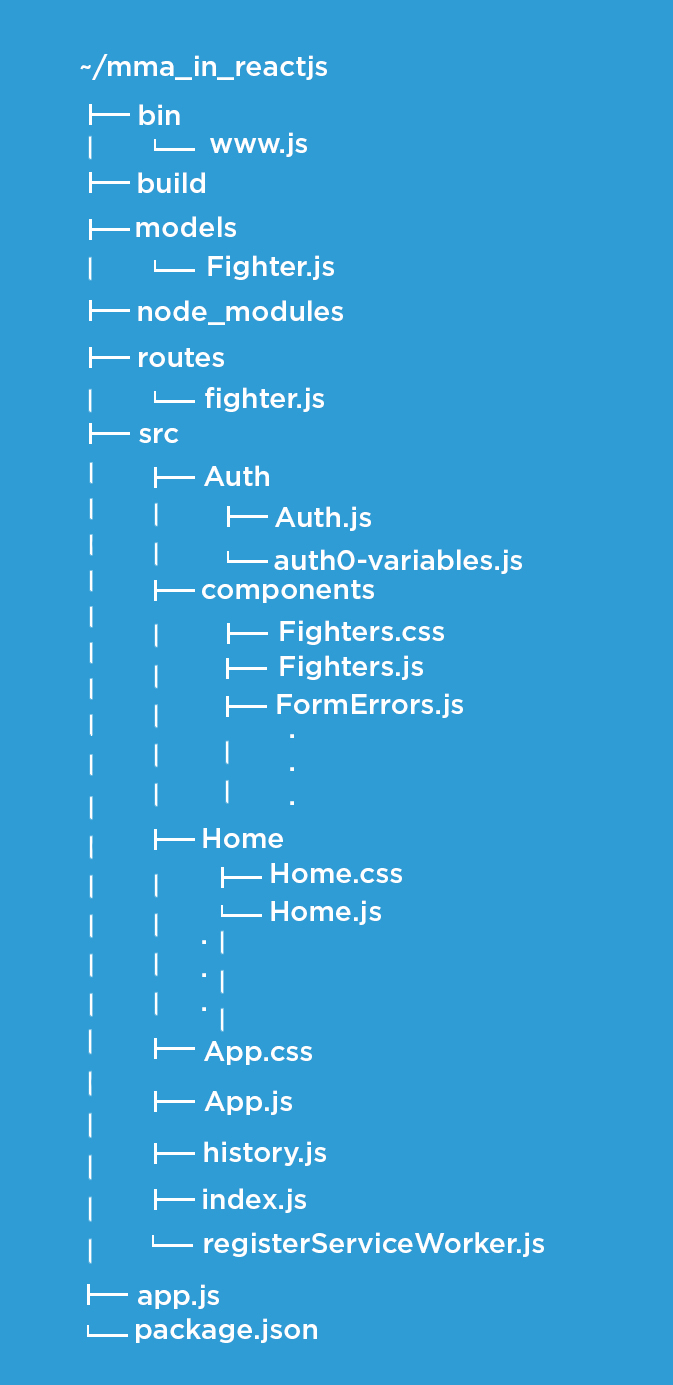
\includegraphics[scale=0.7]{kepek/mma_in_reactjs.jpeg}
\caption{A ReactJS projekt struktúrája}
\label{fig:reactjs_structure}
\end{figure}
